\documentclass{standalone}

%----------------------------------------------------------------------------------------------%
%                                 Packages and basic declarations
%----------------------------------------------------------------------------------------------%

\usepackage[utf8]{inputenc}
\usepackage{pgfplots}
\usepackage{tikz}


%----------------------------------------------------------------------------------------------%
%----------------------------------------------------------------------------------------------%
%                                            DOCUMENT STARTS
%----------------------------------------------------------------------------------------------%
%----------------------------------------------------------------------------------------------%

\begin{document}


%Tikz picture starts%

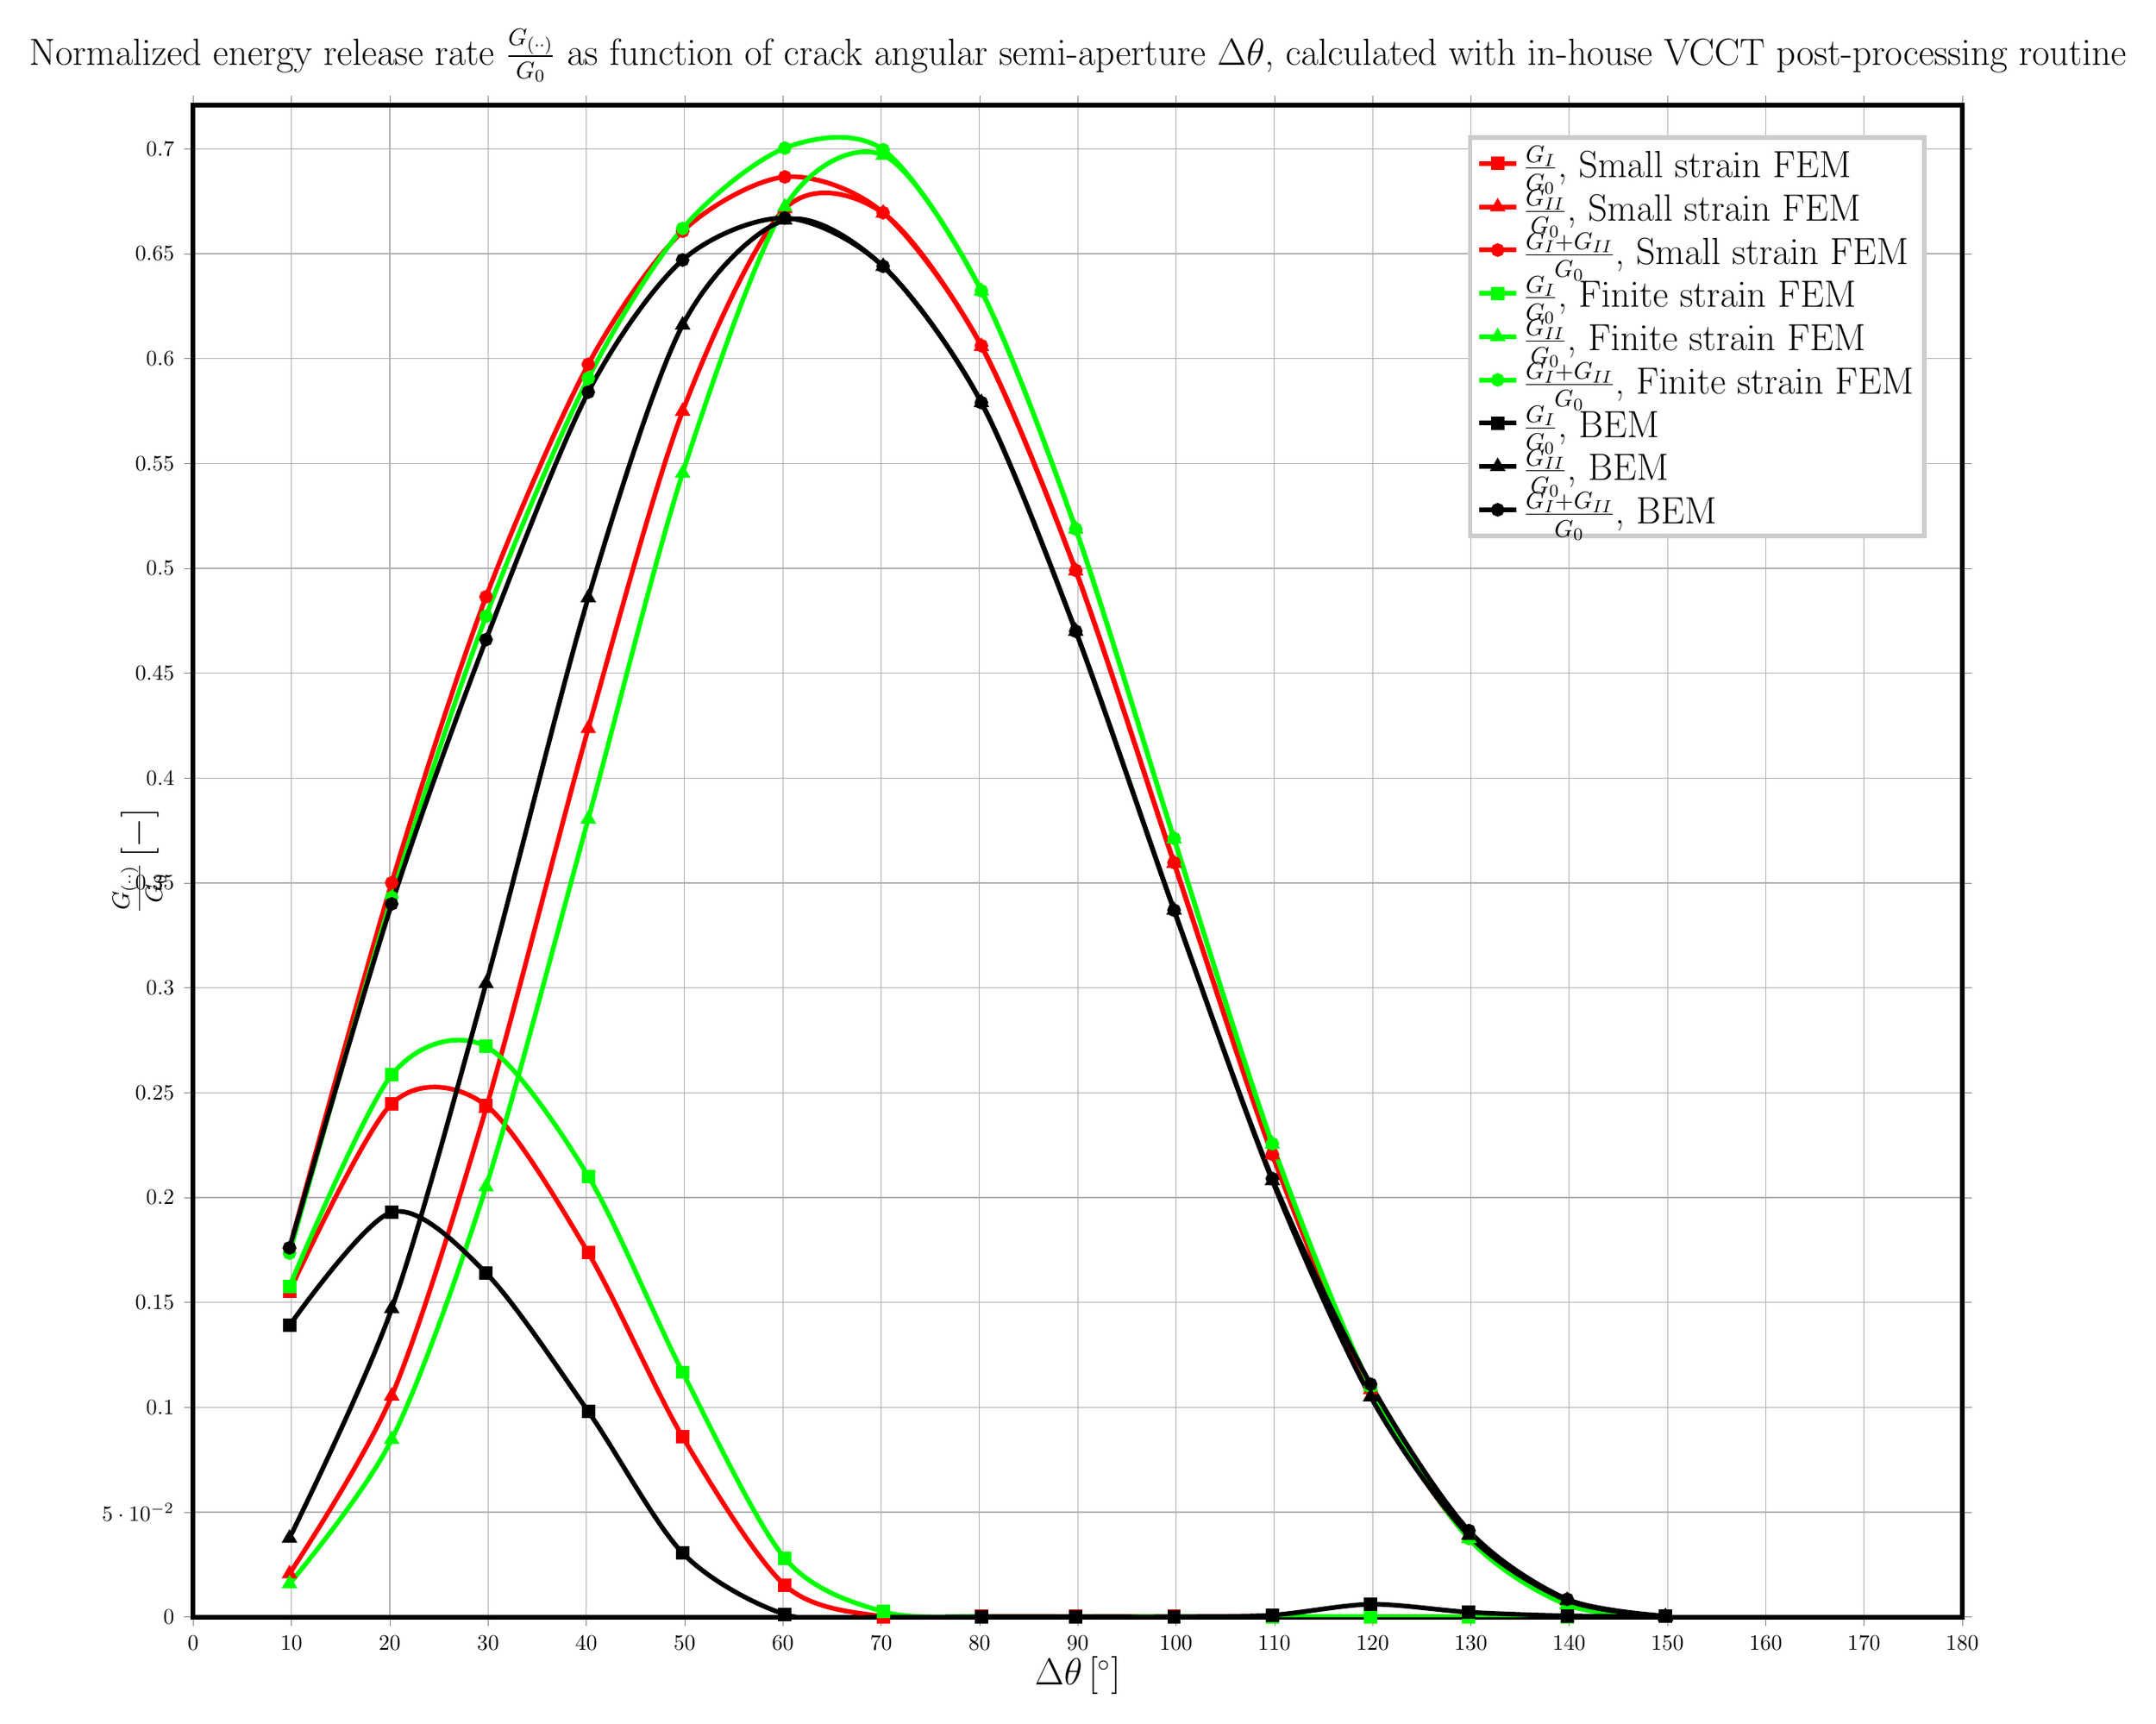
\begin{tikzpicture}

%Tikz axis starts%

\begin{axis}[width=30cm,
title={Normalized energy release rate $\frac{G_{\left(\cdot\cdot\right)}}{G_{0}}$ as function of crack angular semi-aperture  $\Delta\theta$, calculated with in-house VCCT post-processing routine},
title style={font=\fontsize{16}{8}\selectfont},
xlabel style={at={(axis description cs:0.5,-0.02)},anchor=north,font=\fontsize{16}{8}\selectfont},
ylabel style={at={(axis description cs:-0.01,.5)},anchor=south,font=\fontsize{16}{8}\selectfont},
xlabel={$\Delta\theta\left[^{\circ}\right]$},ylabel={$\frac{G_{\left(\cdot\cdot\right)}}{G_{0}}\left[-\right]$},
xmin=0.0,
xmax=180.0,
ymin=0.0,
ymax=0.720949567391,
tick align=outside,
xtick={0.0,10.0,20.0,30.0,40.0,50.0,60.0,70.0,80.0,90.0,100.0,110.0,120.0,130.0,140.0,150.0,160.0,170.0,180.0},
xmajorgrids,
x grid style={lightgray!92.026143790849673!black},
ymajorgrids,
y grid style={lightgray!92.026143790849673!black},
tick label style={font=\normalsize},
line width=0.75mm,
legend style={draw=white!80.0!black,font=\fontsize{16}{12}\selectfont},
legend entries={{$\frac{G_{I}}{G_{0}}$, Small strain FEM},{$\frac{G_{II}}{G_{0}}$, Small strain  FEM},{$\frac{G_{I}+G_{II}}{G_{0}}$, Small strain  FEM},{$\frac{G_{I}}{G_{0}}$, Finite strain FEM},{$\frac{G_{II}}{G_{0}}$, Finite strain  FEM},{$\frac{G_{I}+G_{II}}{G_{0}}$, Finite strain  FEM},{$\frac{G_{I}}{G_{0}}$, BEM},{$\frac{G_{II}}{G_{0}}$, BEM},{$\frac{G_{I}+G_{II}}{G_{0}}$, BEM}},
legend cell align={left}
]

\addplot[red,smooth,mark=square*]
table{
9.8000083551 0.155279714464
20.2001564043 0.244682227012
29.7996713865 0.243940325599
40.1999526243 0.173634167537
49.8000464651 0.085835685135
60.2003242878 0.0151498656859
70.1998714969 0.000211123676354
80.1999924418 0.000340824202666
89.799994075 0.000245127286501
99.8000057369 0.000349689061313
109.800126682 0.000234111719655
119.799673891 0.000144611932243
129.800136345 4.31366251995e-05
139.800052385 8.57513371802e-06
149.799859141 0.000343559987518
};

\addplot[red,smooth,mark=triangle*]
table{
9.8000083551 0.0206235682795
20.2001564043 0.105372101051
29.7996713865 0.242490141025
40.1999526243 0.423625397235
49.8000464651 0.574881076847
60.2003242878 0.671468769924
70.1998714969 0.669359474636
80.1999924418 0.605804351616
89.799994075 0.498764935444
99.8000057369 0.359338306179
109.800126682 0.220354671371
119.799673891 0.108432625938
129.800136345 0.0374607919239
139.800052385 0.00596610490669
149.799859141 5.26625371324e-05
};

\addplot[red,smooth,mark=*]
table{
9.8000083551 0.175903282743
20.2001564043 0.350054328063
29.7996713865 0.486430466624
40.1999526243 0.597259564772
49.8000464651 0.660716761982
60.2003242878 0.68661863561
70.1998714969 0.669570598312
80.1999924418 0.606145175819
89.799994075 0.49901006273
99.8000057369 0.35968799524
109.800126682 0.22058878309
119.799673891 0.10857723787
129.800136345 0.0375039285491
139.800052385 0.00597468004041
149.799859141 0.00039622252465
};

\addplot[green,smooth,mark=square*]
table{
9.8000083551 0.157625277795
20.2001564043 0.258483375809
29.7996713865 0.272053352564
40.1999526243 0.210152492351
49.8000464651 0.116696866394
60.2003242878 0.028009443926
70.1998714969 0.00257274668203
80.1999924418 0.000174246072117
89.799994075 7.34158413423e-05
99.8000057369 0.000221111832752
109.800126682 0.000234812763978
119.799673891 0.000167595874307
129.800136345 5.85937939603e-05
139.800052385 1.03236833497e-05
149.799859141 0.00036235858838
};

\addplot[green,smooth,mark=triangle*]
table{
9.8000083551 0.0158327218093
20.2001564043 0.0846675619162
29.7996713865 0.205131412386
40.1999526243 0.380466865897
49.8000464651 0.545349492415
60.2003242878 0.672342586549
70.1998714969 0.69699018236
80.1999924418 0.63213498481
89.799994075 0.518678842284
99.8000057369 0.371002901206
109.800126682 0.225422718435
119.799673891 0.109725861563
129.800136345 0.0374157324093
139.800052385 0.00583528656526
149.799859141 6.47298931743e-05
};

\addplot[green,smooth,mark=*]
table{
9.8000083551 0.173457999604
20.2001564043 0.343150937726
29.7996713865 0.47718476495
40.1999526243 0.590619358249
49.8000464651 0.662046358809
60.2003242878 0.700352030475
70.1998714969 0.699562929042
80.1999924418 0.632309230883
89.799994075 0.518752258125
99.8000057369 0.371224013039
109.800126682 0.225657531199
119.799673891 0.109893457437
129.800136345 0.0374743262033
139.800052385 0.00584561024861
149.799859141 0.000427088481554
};

\addplot[black,smooth,mark=square*]
table{
9.8000083551 0.139
20.2001564043 0.193
29.7996713865 0.164
40.1999526243 0.098
49.8000464651 0.0305
60.2003242878 0.00127
70.1998714969 -4.79e-05
80.1999924418 6.85e-05
89.799994075 0.000112
99.8000057369 0.000112
109.800126682 0.000895
119.799673891 0.00607
129.800136345 0.00229
139.800052385 0.000552
149.799859141 0.000306
};

\addplot[black,smooth,mark=triangle*]
table{
9.8000083551 0.0376
20.2001564043 0.147
29.7996713865 0.302
40.1999526243 0.486
49.8000464651 0.616
60.2003242878 0.666
70.1998714969 0.644
80.1999924418 0.579
89.799994075 0.47
99.8000057369 0.337
109.800126682 0.208
119.799673891 0.105
129.800136345 0.0389
139.800052385 0.00792
149.799859141 0.000165
};

\addplot[black,smooth,mark=*]
table{
9.8000083551 0.176
20.2001564043 0.34
29.7996713865 0.466
40.1999526243 0.584
49.8000464651 0.647
60.2003242878 0.667
70.1998714969 0.644
80.1999924418 0.579
89.799994075 0.47
99.8000057369 0.337
109.800126682 0.209
119.799673891 0.111
129.800136345 0.0412
139.800052385 0.00847
149.799859141 0.000471
};

\end{axis}
%Tikz axis ends%


\end{tikzpicture}
%Tikz picture ends%


\end{document}

%----------------------------------------------------------------------------------------------%
%----------------------------------------------------------------------------------------------%
%                                            DOCUMENT ENDS
%----------------------------------------------------------------------------------------------%
%----------------------------------------------------------------------------------------------%

